\documentclass{homeworg}
\usepackage{threeparttable}
\usepackage{lscape}
\usepackage{natbib}
\usepackage{graphicx}
\usepackage{listings}
\usepackage{caption}
\usepackage{subcaption}
\usepackage{booktabs}
\usepackage{hyperref}
\usepackage{float}



\title{Bayesian Statistics Final}
\author{Weijia Zhao}



\begin{document}
\maketitle

\textbf{Caution:} I keep 6 decimal digits for infinite decimals.

\exercise 
\textbf{Orthodontic Distance} \\
Measurements on 16 boys and 11 girls with the random effect model d (i=1,...27; j=1,..4)
\begin{align*}
y_{ij}|\beta_0, \beta_1, \beta_2, u_i, \sigma_\epsilon^2 & \sim^{ind} N(\beta_0+\beta_1 age_{ij}+\beta_2sex_i+u_i,\sigma_\epsilon^2)\\
u_i|\sigma_u^2 & \sim^{iid} N(0,\sigma_u^2)
\end{align*}
Assume the prior distributions 
\begin{align*}
\beta_k &\sim^{iid} N(0,\sigma^2=10^8), k=0,1,1\\
\tau_\epsilon & \sim Gamma(0.01,0.01)\\
\tau_u & \sim Gamma(0.01,0.01)
\end{align*}

(1) The random effects model is given as following\footnote{For the random effect model, we need to introduce 27 random variables $u_i$ and each of them represents the random effect for one individual child and is associated with 4 observations}

\begin{table}[H]
	\caption{Q1(a) Regression Results}
	\begin{tabular}{llllllllll}
		\hline \hline
		& mean   & sd    & hdi\_2.5\% & hdi\_97.5\% & mcse\_mean & mcse\_sd & ess\_bulk & ess\_tail & r\_hat \\ \hline
		beta1{[}0{]} & 16.545 & 0.794 & 14.992     & 18.111      & 0.002      & 0.001    & 161707.0  & 233967.0  & 1.0    \\
		beta1{[}1{]} & 0.66   & 0.063 & 0.537      & 0.782       & 0.0        & 0.0      & 290661.0  & 286379.0  & 1.0    \\
		beta1{[}2{]} & 1.16   & 0.395 & 0.376      & 1.934       & 0.001      & 0.001    & 75108.0   & 125895.0  & 1.0    \\
		u1{[}M01{]}  & 2.388  & 0.812 & 0.785      & 3.981       & 0.002      & 0.001    & 176479.0  & 226593.0  & 1.0    \\
		u1{[}M02{]}  & -1.368 & 0.806 & -2.947     & 0.221       & 0.002      & 0.001    & 178175.0  & 230411.0  & 1.0    \\
		u1{[}M03{]}  & -0.619 & 0.803 & -2.185     & 0.971       & 0.002      & 0.001    & 185712.0  & 239467.0  & 1.0    \\
		u1{[}M04{]}  & 1.421  & 0.805 & -0.168     & 2.999       & 0.002      & 0.001    & 181921.0  & 235212.0  & 1.0    \\
		u1{[}M05{]}  & -1.691 & 0.807 & -3.279     & -0.104      & 0.002      & 0.001    & 182685.0  & 232680.0  & 1.0    \\
		u1{[}M06{]}  & 1.207  & 0.806 & -0.369     & 2.795       & 0.002      & 0.001    & 181590.0  & 236442.0  & 1.0    \\
		u1{[}M07{]}  & -1.047 & 0.804 & -2.63      & 0.527       & 0.002      & 0.001    & 184612.0  & 233608.0  & 1.0    \\
		u1{[}M08{]}  & -0.94  & 0.804 & -2.497     & 0.667       & 0.002      & 0.001    & 182287.0  & 233078.0  & 1.0    \\
		u1{[}M09{]}  & 0.133  & 0.802 & -1.443     & 1.713       & 0.002      & 0.001    & 183884.0  & 237202.0  & 1.0    \\
		u1{[}M10{]}  & 3.889  & 0.83  & 2.283      & 5.542       & 0.002      & 0.001    & 190979.0  & 233895.0  & 1.0    \\
		u1{[}M11{]}  & -1.155 & 0.805 & -2.719     & 0.441       & 0.002      & 0.001    & 186663.0  & 234630.0  & 1.0    \\
		u1{[}M12{]}  & -0.616 & 0.801 & -2.202     & 0.944       & 0.002      & 0.001    & 189475.0  & 238159.0  & 1.0    \\
		u1{[}M13{]}  & -0.618 & 0.801 & -2.193     & 0.957       & 0.002      & 0.001    & 189113.0  & 238027.0  & 1.0    \\
		u1{[}M14{]}  & -0.081 & 0.802 & -1.649     & 1.504       & 0.002      & 0.001    & 182420.0  & 239946.0  & 1.0    \\
		u1{[}M15{]}  & 0.778  & 0.804 & -0.783     & 2.368       & 0.002      & 0.001    & 192143.0  & 235755.0  & 1.0    \\
		u1{[}M16{]}  & -1.691 & 0.809 & -3.298     & -0.121      & 0.002      & 0.001    & 185518.0  & 232355.0  & 1.0    \\
		u1{[}F01{]}  & -1.094 & 0.856 & -2.778     & 0.594       & 0.002      & 0.002    & 157014.0  & 218335.0  & 1.0    \\
		u1{[}F02{]}  & 0.304  & 0.855 & -1.381     & 1.982       & 0.002      & 0.002    & 156281.0  & 223321.0  & 1.0    \\
		u1{[}F03{]}  & 0.946  & 0.855 & -0.743     & 2.619       & 0.002      & 0.002    & 155958.0  & 221905.0  & 1.0    \\
		u1{[}F04{]}  & 1.912  & 0.863 & 0.22       & 3.605       & 0.002      & 0.002    & 159540.0  & 215766.0  & 1.0    \\
		u1{[}F05{]}  & -0.019 & 0.855 & -1.695     & 1.658       & 0.002      & 0.002    & 160283.0  & 225459.0  & 1.0    \\
		u1{[}F06{]}  & -1.307 & 0.859 & -3.005     & 0.367       & 0.002      & 0.002    & 152668.0  & 214479.0  & 1.0    \\
		u1{[}F07{]}  & 0.302  & 0.855 & -1.376     & 1.991       & 0.002      & 0.002    & 155892.0  & 218599.0  & 1.0    \\
		u1{[}F08{]}  & 0.625  & 0.856 & -1.066     & 2.304       & 0.002      & 0.002    & 152895.0  & 221492.0  & 1.0    \\
		u1{[}F09{]}  & -1.308 & 0.859 & -3.009     & 0.367       & 0.002      & 0.002    & 155090.0  & 213259.0  & 1.0    \\
		u1{[}F10{]}  & -3.562 & 0.876 & -5.297     & -1.861      & 0.002      & 0.002    & 153914.0  & 210689.0  & 1.0    \\
		u1{[}F11{]}  & 3.198  & 0.874 & 1.517      & 4.944       & 0.002      & 0.002    & 157232.0  & 207386.0  & 1.0    \\
		tau\_e1      & 0.486  & 0.077 & 0.341      & 0.641       & 0.0        & 0.0      & 357083.0  & 300452.0  & 1.0    \\
		tau\_u1      & 0.318  & 0.108 & 0.132      & 0.534       & 0.0        & 0.0      & 301027.0  & 273672.0  & 1.0    \\
		rho1         & 0.611  & 0.089 & 0.435      & 0.779       & 0.0        & 0.0      & 293524.0  & 285156.0  & 1.0   \\
		sigmae2 & 2.11 & 0.343 & 1.483 & 2.794 & 0.001 & 0.0 & 357083.0 & 300452.0 & 1.0 \\
		 \hline\hline
	\end{tabular}
\end{table}

\begin{figure}[H]
	\caption{Q1(a) Parameter Histogram}
\begin{subfigure}{0.48\textwidth}
	\centering
	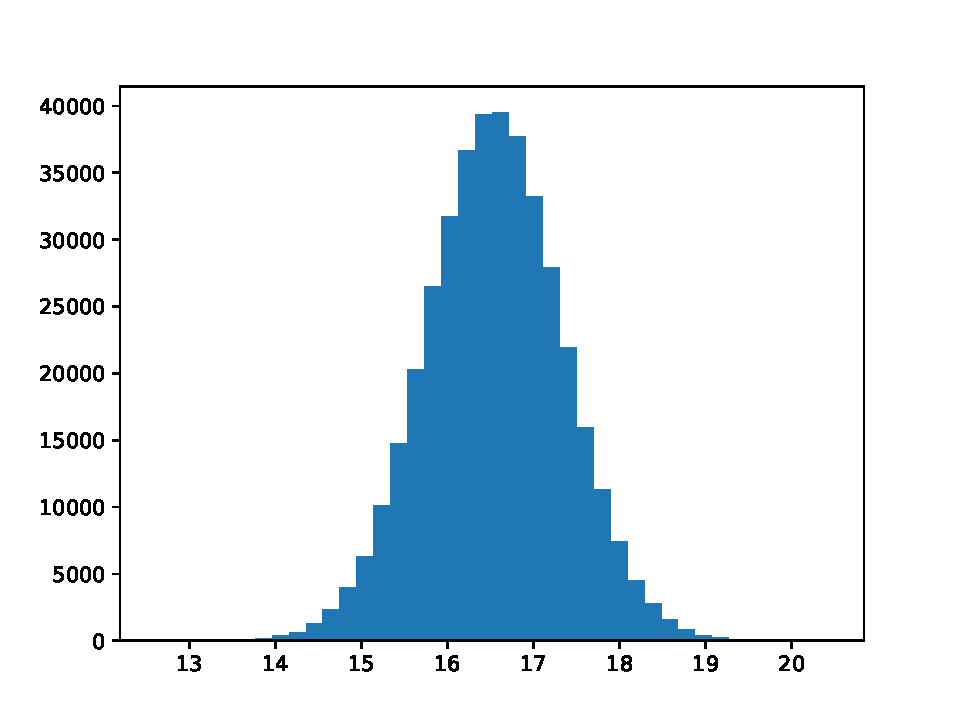
\includegraphics[width=\textwidth]{q1_a_beta0.pdf}
	\caption{Q1a) Distribution of $\beta_0$}
\end{subfigure}
\begin{subfigure}{0.48\textwidth}
	\centering
	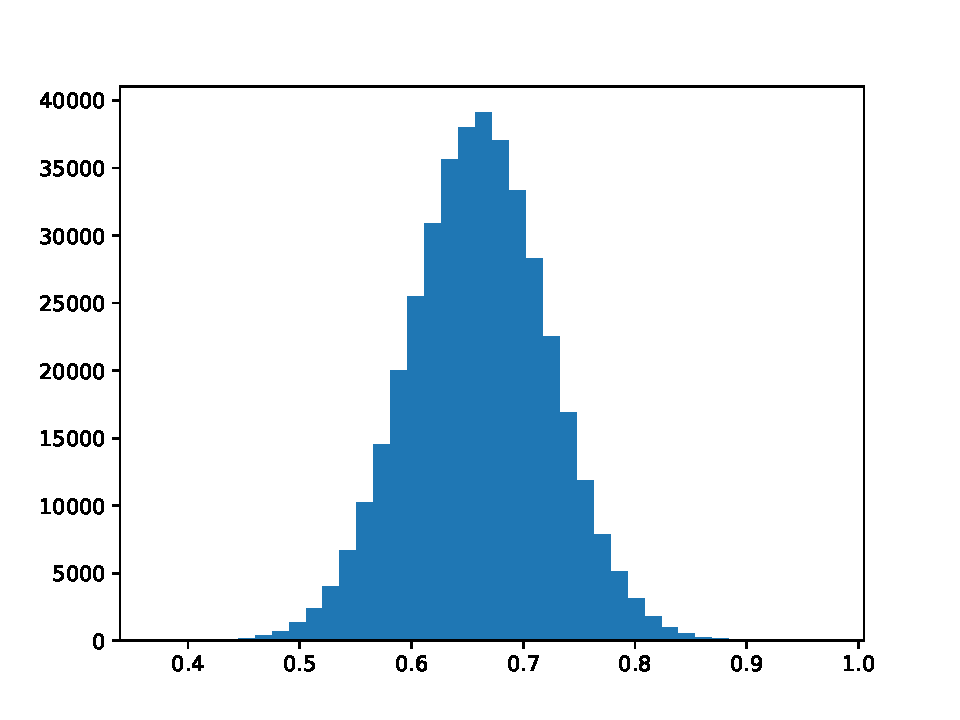
\includegraphics[width=\textwidth]{q1_a_beta1.pdf}
	\caption{(Q1a) Distribution of $\beta_1$}
\end{subfigure}
	\begin{subfigure}{0.48\textwidth}
	\centering
	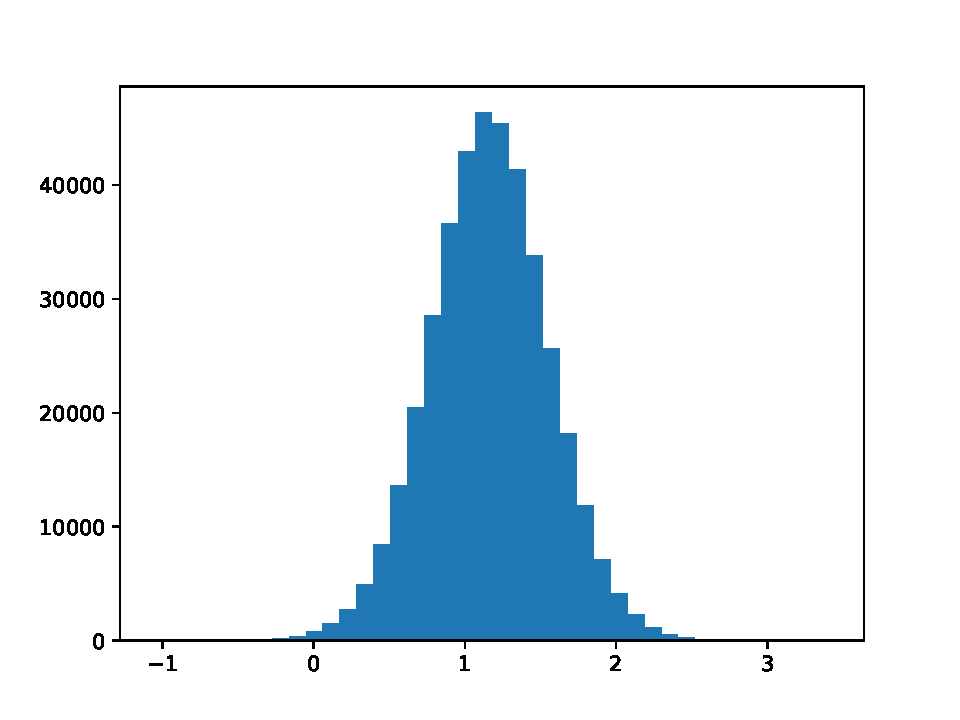
\includegraphics[width=\textwidth]{q1_a_beta2.pdf}
	\caption{(Q1a) Distribution of $\beta_2$}
\end{subfigure}
\begin{subfigure}{0.48\textwidth}
	\centering
	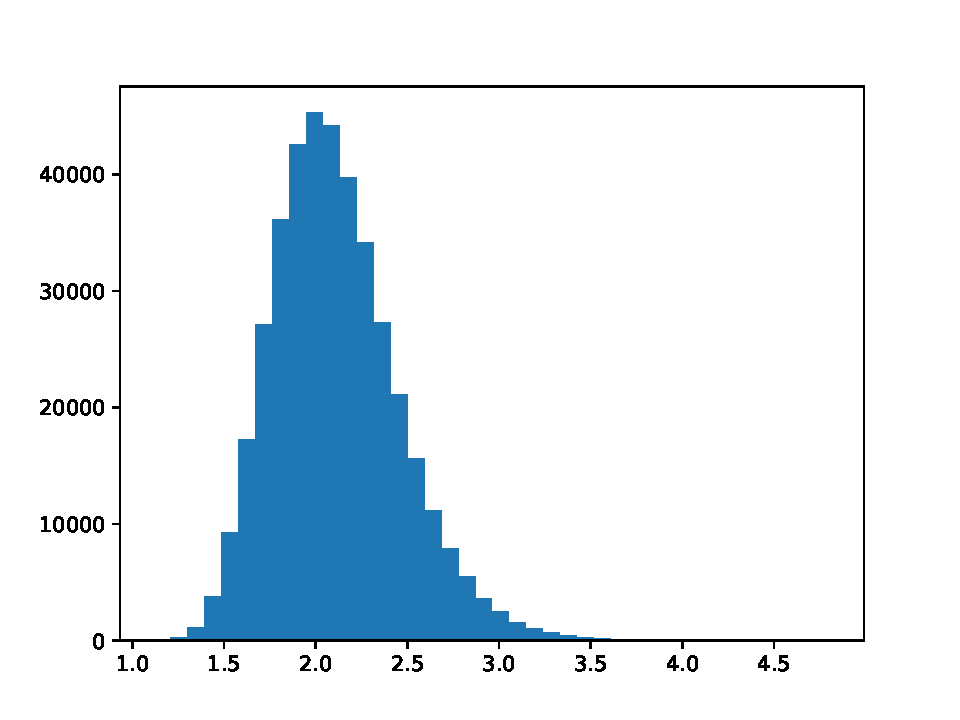
\includegraphics[width=\textwidth]{q1_a_sigmae.pdf}
	\caption{(Q1a) Distribution of $\sigma_\epsilon^2$}
\end{subfigure}
\begin{subfigure}{0.48\textwidth}
	\centering
	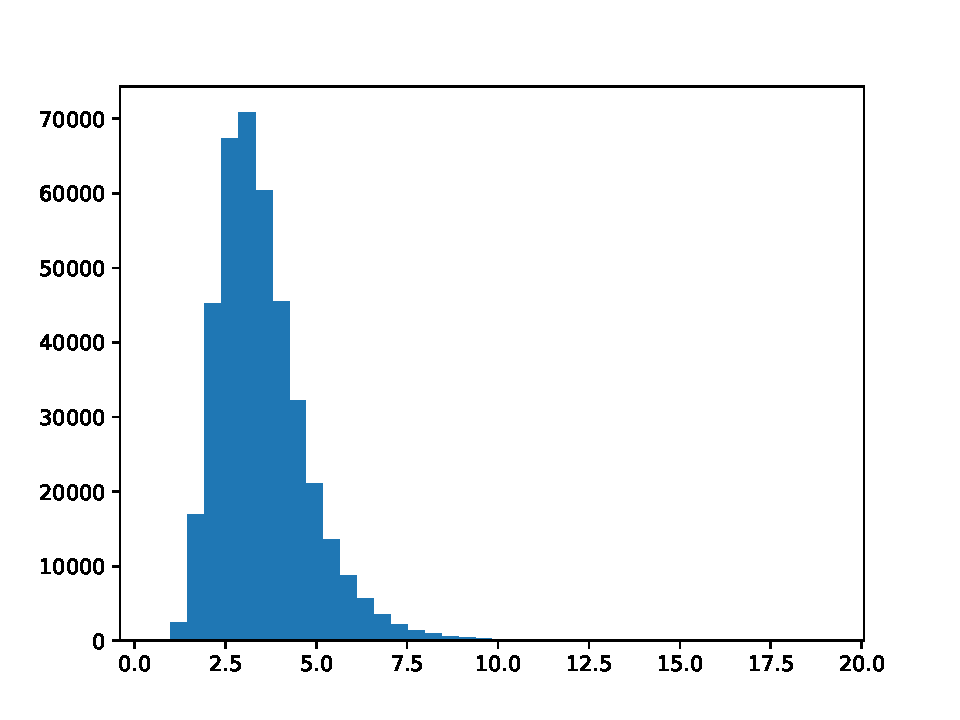
\includegraphics[width=\textwidth]{q1_a_sigmau.pdf}
	\caption{(Q1a) Distribution of $\sigma_u^2$}
\end{subfigure}
\end{figure}




(b) From the results table above, we see that the distribution of $\rho$ has mean 0.611 with 95\% credible set to be $[0.435,0.779]$. Thus it appear to be significantly differently from 0. The histogram of $\rho$ is given below
\begin{figure}[h]
\caption{Q1(b) Parameter Histogram}
\begin{subfigure}[b]{0.48\textwidth}
\centering
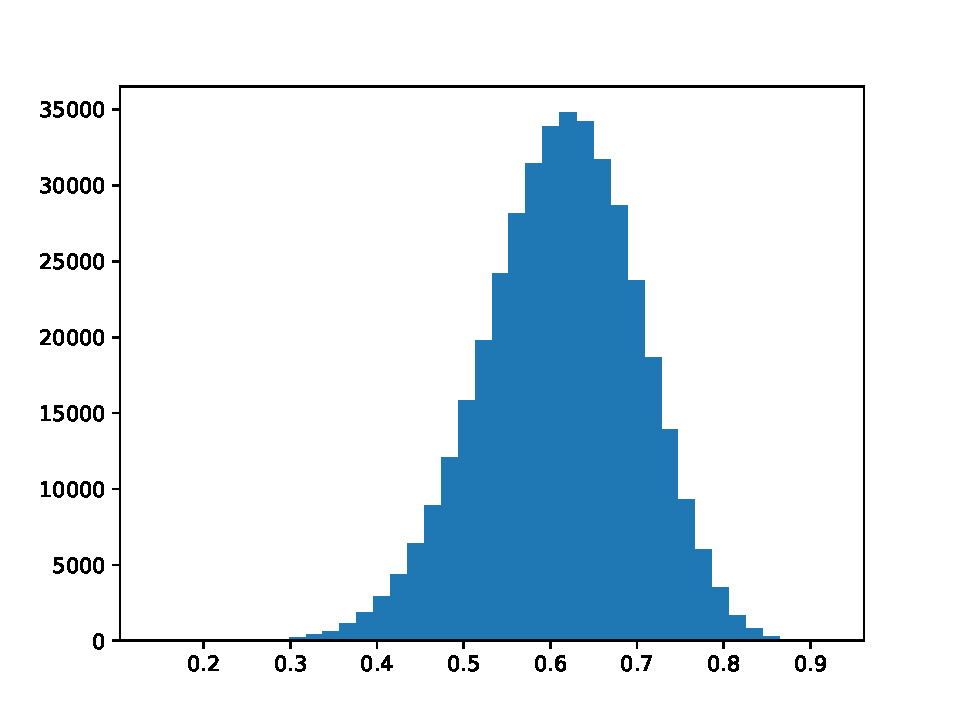
\includegraphics[width=\textwidth]{q1_b_rho.pdf}
\caption{(Q1b) Distribution of $\rho$}
\end{subfigure}
\end{figure}

(c) The model results and the posterior densities of those parameters are given as following. 
\begin{itemize}
\item For $\beta_0$, with random effect, the mean is 16.545 with 95\% credible set $[14.992,18.111]$, without random effect, the mean is 16.532 with 95\% credible set $[14.335,18.694]$
\item For $\beta_1$, with random effect, the mean is 0.66 with 95\% credible set $[0.537,0.782]$ and without random effect, the mean is 0.661 with 95\% credible set $[0.467,0.855]$
\item For $\beta_2$, with random effect, the mean is 1.16 with 95\% credible set $[0.376,1.934]$ and without random effect, the mean is 1.161 with 95\% credible set 
$[0.719,1.599]$
\item For $\sigma_\epsilon^2$, with random effect, the mean is 2.11 with 95\% credible set $[1.483,2.794]$ and without random effect, the mean is 5.253 with 95\% credible set to be $[3.902,6.735]$
\end{itemize}
The estimation of $\beta$ are pretty close in terms of mean when we include the random effect or not include. The estimation of $\sigma_\epsilon^2$ is much smaller when we include random effect compared to the model when we do not have random effects. Thus random effects help to reduce the variance of the model.

\begin{table}[H]
		\caption{Q1(c) Regression Results}
	\begin{tabular}{llllllllll}
		\hline \hline
		& mean   & sd    & hdi\_2.5\% & hdi\_97.5\% & mcse\_mean & mcse\_sd & ess\_bulk & ess\_tail & r\_hat \\ \hline
		beta2{[}0{]} & 16.532 & 1.112 & 14.335     & 18.694      & 0.005      & 0.004    & 44165.0   & 68519.0   & 1.0    \\
		beta2{[}1{]} & 0.661  & 0.099 & 0.467      & 0.855       & 0.0        & 0.0      & 44175.0   & 67615.0   & 1.0    \\
		beta2{[}2{]} & 1.161  & 0.224 & 0.719      & 1.599       & 0.001      & 0.001    & 78405.0   & 101859.0  & 1.0    \\
		tau\_e2      & 0.194  & 0.027 & 0.143      & 0.247       & 0.0        & 0.0      & 76023.0   & 104774.0  & 1.0    \\
		tau\_u2      & 1.001  & 8.827 & 0.0        & 0.383       & 0.106      & 0.078    & 34411.0   & 58444.0   & 1.0   \\
		sigmae2 & 5.253 & 0.738 & 3.902 & 6.735 & 0.003 & 0.002 & 76023.0 & 104774.0 &1.0\\
		 \hline\hline
	\end{tabular}
\end{table}

The histogram of parameters are given below
\begin{figure}[H]
		\caption{Q1(c) Parameter Histogram}
	\begin{subfigure}{0.48\textwidth}
		\centering
		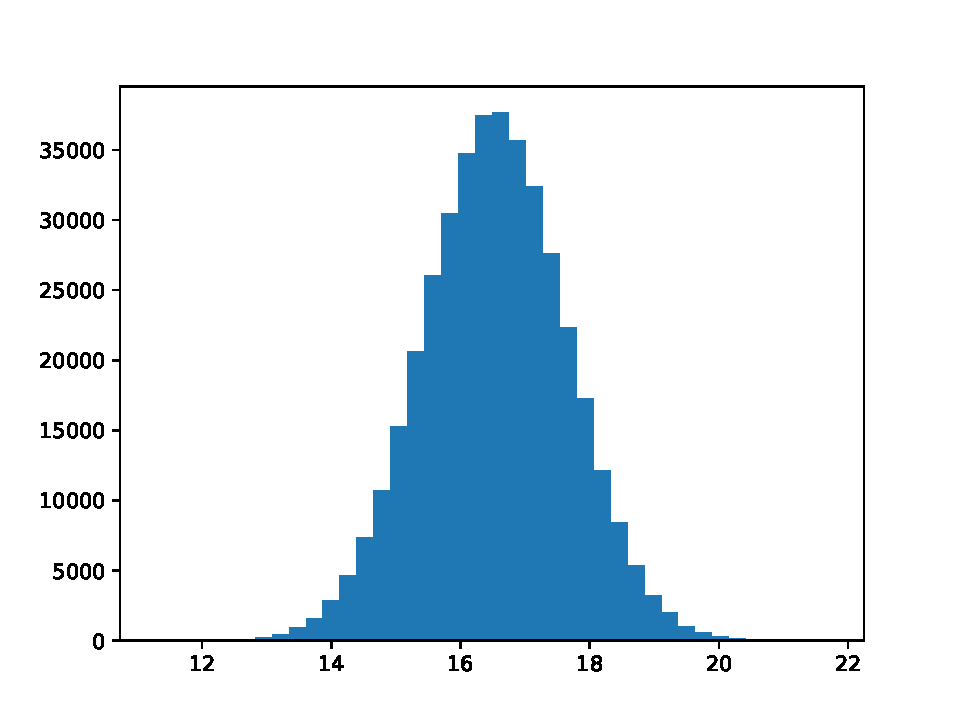
\includegraphics[width=\textwidth]{q1_c_beta0.pdf}
		\caption{(Q1c) Distribution of $\beta_0$}
	\end{subfigure}
	\begin{subfigure}{0.48\textwidth}
		\centering
		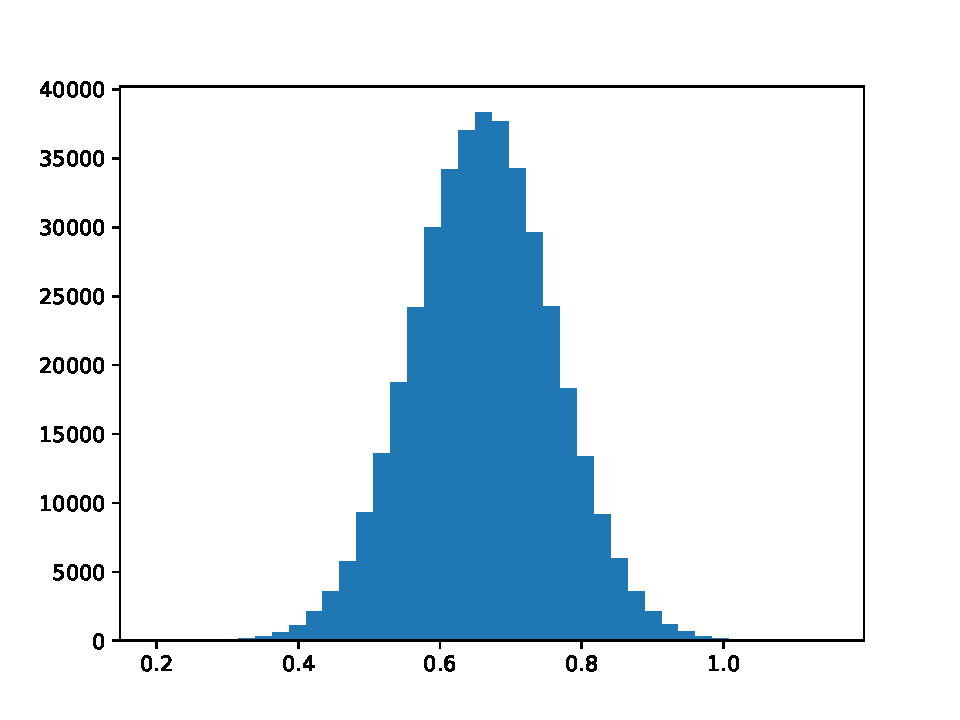
\includegraphics[width=\textwidth]{q1_c_beta1.pdf}
		\caption{(Q1c) Distribution of $\beta_1$}
	\end{subfigure}
	\begin{subfigure}{0.48\textwidth}
	\centering
	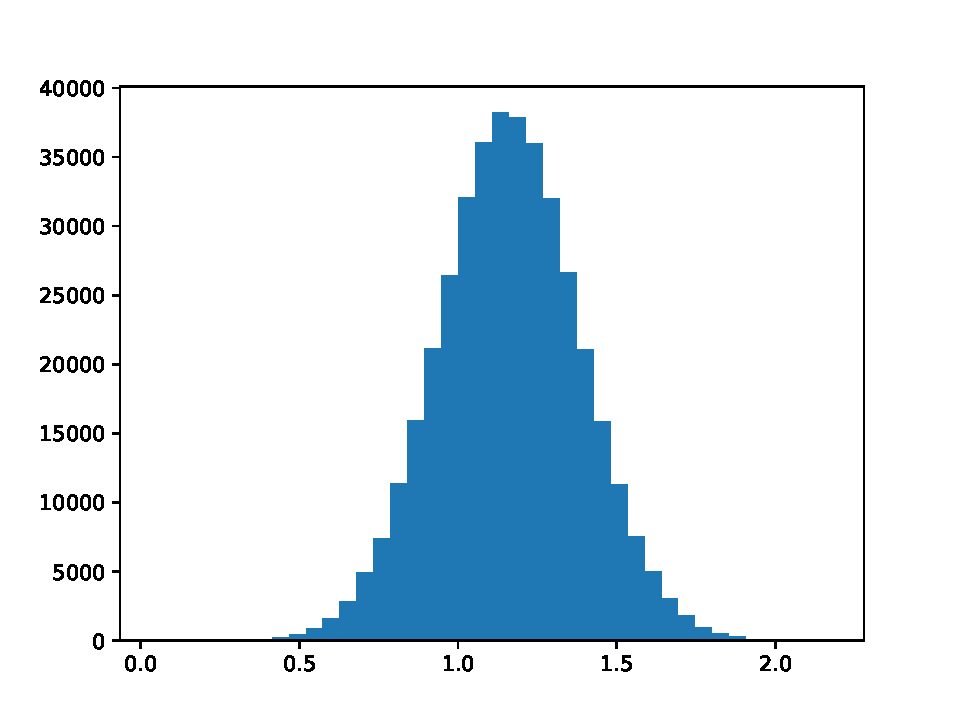
\includegraphics[width=\textwidth]{q1_c_beta2.pdf}
	\caption{(Q1c) Distribution of $\beta_2$}
\end{subfigure}
\begin{subfigure}{0.48\textwidth}
	\centering
	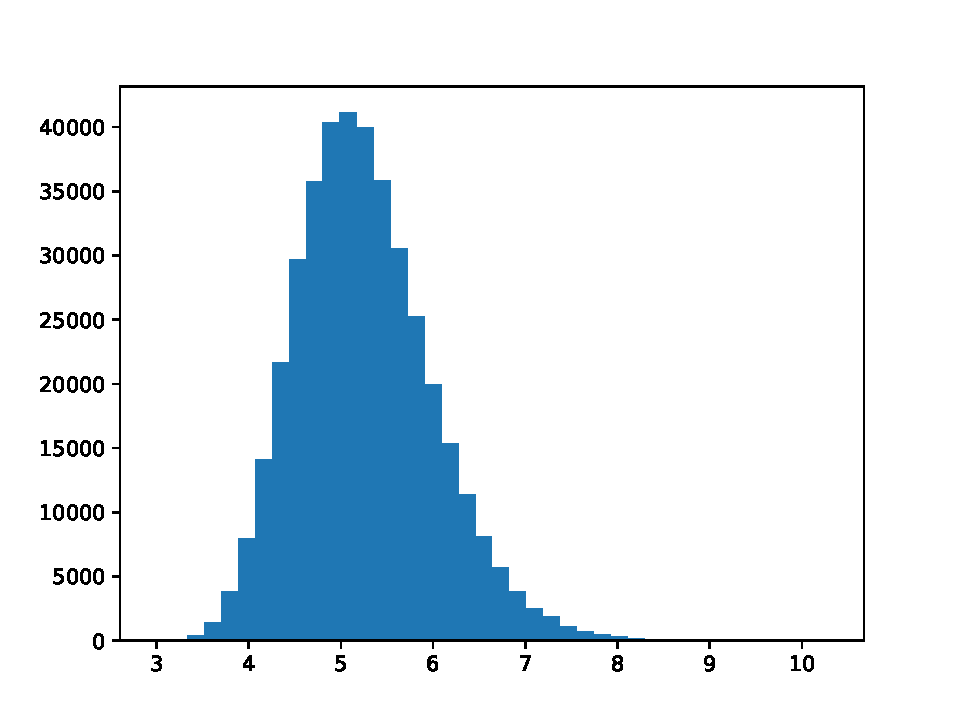
\includegraphics[width=\textwidth]{q1_c_sigmae.pdf}
	\caption{(Q1c) Distribution of $\sigma_\epsilon^2$}
\end{subfigure}
\end{figure}

\exercise 
\textbf{Nanowire Density} \\
The density of nanowires is assumed to follow a Poisson distribution with mean 
\begin{align*}
\mu(x)=\theta_1e^{-\theta_2x^2}+\theta_3(1-e^{-\theta_2x^2})\Phi(-x/\theta_4)
\end{align*}
Assume the prior distribution of parameters to be 
\begin{align*}
\log \theta_1,\log\theta_3,\log\theta_4 & \sim^{iid} N(0,\sigma^2=10)\\
\theta_2\sim U(0,1)
\end{align*}

(a) Notice that in pymc, we can directly use pm.LogNormal to use the log normal distribution rather than defining a random variable following normal distribution and then converting it to log normal by taking exponential function. The regression results are given as following. 
\begin{itemize}
\item $\theta_1$: mean is 122.89 with 95\% credible set to be $[107.517,138.08]$
\item $\theta_2$: mean is 0.134 with 95\% credible set to be $[0.134,0.238]$
\item $\theta_3$: mean is 27.066 with 95\% credible set to be $[13.207, 42.097]$
\item $\theta_4$: mean is 11.573 with 95\% credible set to be $[7.454,16.479]$
\end{itemize}
\begin{table}[H]
	\caption{Q2 (a) Regression results}
	\begin{tabular}{llllllllll}
		\hline \hline
		& mean   & sd    & hdi\_2.5\% & hdi\_97.5\% & mcse\_mean & mcse\_sd & ess\_bulk & ess\_tail & r\_hat \\ \hline
		theta1 & 122.89 & 7.818 & 107.517    & 138.08      & 0.017      & 0.012    & 221497.0  & 240127.0  & 1.0    \\
		theta3 & 27.066 & 7.61  & 13.207     & 42.097      & 0.02       & 0.014    & 143991.0  & 162010.0  & 1.0    \\
		theta4 & 11.573 & 6.727 & 7.454      & 16.479      & 0.025      & 0.017    & 147953.0  & 146002.0  & 1.0    \\
		theta2 & 0.185  & 0.027 & 0.134      & 0.238       & 0.0        & 0.0      & 182799.0  & 223993.0  & 1.0   \\ \hline \hline
	\end{tabular}
\end{table}

(b) The results are given by the following table: the mean is 63.992 with 95\% credible set to be $[44.0,80.0]$
\begin{table}[H]
	\caption{Q2 (b) Regression Results}
	\begin{tabular}{llllllllll}
		\hline \hline
		& mean   & sd    & hdi\_2.5\% & hdi\_97.5\% & mcse\_mean & mcse\_sd & ess\_bulk & ess\_tail & r\_hat \\ \hline
		lld & 63.992 & 9.056 & 44.0       & 80.0        & 0.53       & 0.375    & 291.0     & 733.0     & 1.17  \\ \hline \hline
	\end{tabular}
\end{table}

\exercise 
\textbf{Color Attraction for Oulema Melanopus} \\
To do Bayesian ANOVA analysis, we make the following assumptions: 

We assume the number of insects attracted by each board $y_{ij}$ (for the $jth$ experiment of board $i$) and that 
\begin{align*}
y_{ij} \sim N(\mu_i,\sigma^2)
\mu_i=\mu+\alpha_i
\end{align*}
The null hypothesis is that $H_0: \alpha_1=\alpha_2=\alpha_3=\alpha_4=0$, we use the normalizing specification $\sum_{i=1}^{4}\alpha_i=0$

We use the prior distribution $\alpha_i\sim Normal(0,\tau=0.0001)$ for $i=1,2,3$ where $\tau \sim Gamma(0.001,0.001)$ and $alpha_4$ is determined by the normalizing constraint. 

(a)(b) The ANOVA results are listed as below, here $\alpha_1$ is for lemon yellow board, $\alpha_2$ is for white board, $\alpha_3$ is for green board, $\alpha_4$ is for blue board. Those parameters $diff(ij)$ is for the difference between $\alpha_i$ and $\alpha_j$. As we can see the estimated $mu$ is 27.283 which is the sample average when pool everything together. The estimated $\alpha$s are 19.818, -11.598, -12.449 and 4.228 for yellow, white, green, blue respectively. The difference
\begin{itemize}
\item Yellow-White has mean 31.416 with 95\% credible set $[23.463,39.159]$
\item Yellow-Green has mean 32.267 with 95\% credible set $[23.086,41.092]$
\item Yellow-Blue has mean 15.59 with 95\% credible set $[2.908,27.817]$
\item White-Green has mean 0.851 with 95\% credible set $[-5.673,7.308]$ 
\item White-Blue has mean -15.826 with 95\% credible set $[-26.964,-5.226]$
\item Green-Blue has mean -16.677 with 95\% credible set $[-28.563,-5.138]$
\end{itemize}
We can see Yellow board attracts more compared to any other color board with over 95\% significance. Blue attracts more than White and Green with over 95\% significance. The difference between white and green is slightly positive but not significant since the 95\% credible set almost equally spread over positive and negative region. Thus the overall attractiveness is Lemon Yellow$>$Blue$>$White$\approx$Green
\begin{table}[H]
	\caption{Q3 ANOVA Results}
	\begin{tabular}{llllllllll}
		\hline \hline
		& mean    & sd    & hdi\_2.5\% & hdi\_97.5\% & mcse\_mean & mcse\_sd & ess\_bulk & ess\_tail & r\_hat \\ \hline
		mu         & 27.283  & 1.769 & 23.737     & 30.755      & 0.01       & 0.007    & 33552.0   & 37151.0   & 1.0    \\
		alpha1     & 19.818  & 3.065 & 13.81      & 25.988      & 0.017      & 0.012    & 35756.0   & 35916.0   & 1.0    \\
		alpha2     & -11.598 & 2.151 & -15.952    & -7.421      & 0.012      & 0.008    & 36040.0   & 38629.0   & 1.0    \\
		alpha3     & -12.449 & 2.689 & -17.751    & -7.21       & 0.016      & 0.011    & 37643.0   & 37841.0   & 1.0    \\
		alpha4     & 4.228   & 4.075 & -3.886     & 12.257      & 0.023      & 0.019    & 39066.0   & 35161.0   & 1.0    \\
		diff12     & 31.416  & 3.938 & 23.463     & 39.159      & 0.021      & 0.015    & 38553.0   & 34548.0   & 1.0    \\
		diff13     & 32.267  & 4.534 & 23.086     & 41.092      & 0.026      & 0.019    & 34793.0   & 33589.0   & 1.0    \\
		diff14     & 15.59   & 6.275 & 2.908      & 27.817      & 0.034      & 0.025    & 37525.0   & 36397.0   & 1.0    \\
		diff23     & 0.851   & 3.328 & -5.673     & 7.308       & 0.019      & 0.024    & 43704.0   & 38345.0   & 1.0    \\
		diff24     & -15.826 & 5.457 & -26.964    & -5.226      & 0.03       & 0.023    & 38762.0   & 35472.0   & 1.0    \\
		diff34     & -16.677 & 5.928 & -28.563    & -5.138      & 0.033      & 0.025    & 38615.0   & 35514.0   & 1.0    \\
		tau{[}0{]} & 0.022   & 0.014 & 0.001      & 0.049       & 0.0        & 0.0      & 42421.0   & 32936.0   & 1.0    \\
		tau{[}1{]} & 0.091   & 0.057 & 0.006      & 0.202       & 0.0        & 0.0      & 53740.0   & 38587.0   & 1.0    \\
		tau{[}2{]} & 0.035   & 0.022 & 0.002      & 0.079       & 0.0        & 0.0      & 46801.0   & 33274.0   & 1.0    \\
		tau{[}3{]} & 0.01    & 0.006 & 0.001      & 0.023       & 0.0        & 0.0      & 48468.0   & 35639.0   & 1.0      \\ \hline \hline
	\end{tabular}
\end{table}


%\setlength\bibsep{0pt}
%\bibliographystyle{apalike}
%\bibliography{hw1}

\newpage
\textbf{Q1}
\lstinputlisting[language=Python]{q1.py}
\newpage
\textbf{Q2}
\lstinputlisting[language=Python]{q2.py}
\newpage
\textbf{Q3}
\lstinputlisting[language=Python]{q3.py}
%\lstinputlisting[]{Untitled.do}

\end{document}








